% Created 2021-05-04 Tue 23:43
% Intended LaTeX compiler: pdflatex
\documentclass[12pt]{article}

%%%% settings when exporting code %%%% 

\usepackage{listings}
\lstdefinestyle{code-small}{
backgroundcolor=\color{white}, % background color for the code block
basicstyle=\ttfamily\small, % font used to display the code
commentstyle=\color[rgb]{0.5,0,0.5}, % color used to display comments in the code
keywordstyle=\color{black}, % color used to highlight certain words in the code
numberstyle=\ttfamily\tiny\color{gray}, % color used to display the line numbers
rulecolor=\color{black}, % color of the frame
stringstyle=\color[rgb]{0,.5,0},  % color used to display strings in the code
breakatwhitespace=false, % sets if automatic breaks should only happen at whitespace
breaklines=true, % sets automatic line breaking
columns=fullflexible,
frame=single, % adds a frame around the code (non,leftline,topline,bottomline,lines,single,shadowbox)
keepspaces=true, % % keeps spaces in text, useful for keeping indentation of code
literate={~}{$\sim$}{1}, % symbol properly display via latex
numbers=none, % where to put the line-numbers; possible values are (none, left, right)
numbersep=10pt, % how far the line-numbers are from the code
showspaces=false,
showstringspaces=false,
stepnumber=1, % the step between two line-numbers. If it's 1, each line will be numbered
tabsize=1,
xleftmargin=0cm,
emph={anova,apply,class,coef,colnames,colNames,colSums,dim,dcast,for,ggplot,head,if,ifelse,is.na,lapply,list.files,library,logLik,melt,plot,require,rowSums,sapply,setcolorder,setkey,str,summary,tapply},
aboveskip = \medskipamount, % define the space above displayed listings.
belowskip = \medskipamount, % define the space above displayed listings.
lineskip = 0pt} % specifies additional space between lines in listings
\lstset{style=code-small}
%%%% packages %%%%%

\usepackage[utf8]{inputenc}
\usepackage[T1]{fontenc}
\usepackage{lmodern}
\usepackage{textcomp}
\usepackage{color}
\usepackage{graphicx}
\usepackage{grffile}
\usepackage{wrapfig}
\usepackage{rotating}
\usepackage{longtable}
\usepackage{multirow}
\usepackage{multicol}
\usepackage{changes}
\usepackage{pdflscape}
\usepackage{geometry}
\usepackage[normalem]{ulem}
\usepackage{amssymb}
\usepackage{amsmath}
\usepackage{amsfonts}
\usepackage{dsfont}
\usepackage{array}
\usepackage{ifthen}
\usepackage{hyperref}
\usepackage{natbib}
\RequirePackage{setspace} % to modify the space between lines - incompatible with footnote in beamer
\renewcommand{\baselinestretch}{1.1}
\geometry{top=1cm}
\usepackage{titlesec}
\usepackage{etoolbox}

\makeatletter
\patchcmd{\ttlh@hang}{\parindent\z@}{\parindent\z@\leavevmode}{}{}
\patchcmd{\ttlh@hang}{\noindent}{}{}{}
\makeatother
\RequirePackage{colortbl} % arrayrulecolor to mix colors
\definecolor{myorange}{rgb}{1,0.2,0}
\definecolor{mypurple}{rgb}{0.7,0,8}
\definecolor{mycyan}{rgb}{0,0.6,0.6}
\newcommand{\lightblue}{blue!50!white}
\newcommand{\darkblue}{blue!80!black}
\newcommand{\darkgreen}{green!50!black}
\newcommand{\darkred}{red!50!black}
\definecolor{gray}{gray}{0.5}
\hypersetup{
citecolor=[rgb]{0,0.5,0},
urlcolor=[rgb]{0,0,0.5},
linkcolor=[rgb]{0,0,0.5},
}
\newenvironment{note}{\small \color{gray}\fontfamily{lmtt}\selectfont}{\par}
\newenvironment{activity}{\color{orange}\fontfamily{qzc}\selectfont}{\par}
\RequirePackage{pifont}
\RequirePackage{relsize}
\newcommand{\Cross}{{\raisebox{-0.5ex}%
{\relsize{1.5}\ding{56}}}\hspace{1pt} }
\newcommand{\Valid}{{\raisebox{-0.5ex}%
{\relsize{1.5}\ding{52}}}\hspace{1pt} }
\newcommand{\CrossR}{ \textcolor{red}{\Cross} }
\newcommand{\ValidV}{ \textcolor{green}{\Valid} }
\usepackage{stackengine}
\usepackage{scalerel}
\newcommand\Warning[1][3ex]{%
\renewcommand\stacktype{L}%
\scaleto{\stackon[1.3pt]{\color{red}$\triangle$}{\tiny\bfseries !}}{#1}%
\xspace
}
\newcommand\Rlogo{\textbf{\textsf{R}}\xspace} %
\RequirePackage{fancyvrb}
\DefineVerbatimEnvironment{verbatim}{Verbatim}{fontsize=\small,formatcom = {\color[rgb]{0.5,0,0}}}
\RequirePackage{enumitem} % better than enumerate
\RequirePackage{epstopdf} % to be able to convert .eps to .pdf image files
\RequirePackage{capt-of} %
\RequirePackage{caption} % newlines in graphics
\RequirePackage{tikz-cd} % graph
\RequirePackage{booktabs} % for nice lines in table (e.g. toprule, bottomrule, midrule, cmidrule)
\RequirePackage{amsmath}
\RequirePackage{algorithm}
\RequirePackage[noend]{algpseudocode}
\RequirePackage{dsfont}
\RequirePackage{amsmath,stmaryrd,graphicx}
\RequirePackage{prodint} % product integral symbol (\PRODI)
\usepackage{ifthen}
\usepackage{xifthen}
\usepackage{xargs}
\usepackage{xspace}
\newcommand\defOperator[7]{%
\ifthenelse{\isempty{#2}}{
\ifthenelse{\isempty{#1}}{#7{#3}#4}{#7{#3}#4 \left#5 #1 \right#6}
}{
\ifthenelse{\isempty{#1}}{#7{#3}#4_{#2}}{#7{#3}#4_{#1}\left#5 #2 \right#6}
}
}
\newcommand\defUOperator[5]{%
\ifthenelse{\isempty{#1}}{
#5\left#3 #2 \right#4
}{
\ifthenelse{\isempty{#2}}{\underset{#1}{\operatornamewithlimits{#5}}}{
\underset{#1}{\operatornamewithlimits{#5}}\left#3 #2 \right#4}
}
}
\newcommand{\defBoldVar}[2]{
\ifthenelse{\equal{#2}{T}}{\boldsymbol{#1}}{\mathbf{#1}}
}
\newcommandx\Esp[2][1=,2=]{\defOperator{#1}{#2}{E}{}{\lbrack}{\rbrack}{\mathbb}}
\newcommandx\Prob[2][1=,2=]{\defOperator{#1}{#2}{P}{}{\lbrack}{\rbrack}{\mathbb}}
\newcommandx\Qrob[2][1=,2=]{\defOperator{#1}{#2}{Q}{}{\lbrack}{\rbrack}{\mathbb}}
\newcommandx\Var[2][1=,2=]{\defOperator{#1}{#2}{V}{ar}{\lbrack}{\rbrack}{\mathbb}}
\newcommandx\Cov[2][1=,2=]{\defOperator{#1}{#2}{C}{ov}{\lbrack}{\rbrack}{\mathbb}}
\newcommandx\Binom[2][1=,2=]{\defOperator{#1}{#2}{B}{}{(}{)}{\mathcal}}
\newcommandx\Gaus[2][1=,2=]{\defOperator{#1}{#2}{N}{}{(}{)}{\mathcal}}
\newcommandx\Wishart[2][1=,2=]{\defOperator{#1}{#2}{W}{ishart}{(}{)}{\mathcal}}
\newcommandx\Likelihood[2][1=,2=]{\defOperator{#1}{#2}{L}{}{(}{)}{\mathcal}}
\newcommandx\logLikelihood[2][1=,2=]{\defOperator{#1}{#2}{\ell}{}{(}{)}{}}
\newcommandx\Information[2][1=,2=]{\defOperator{#1}{#2}{I}{}{(}{)}{\mathcal}}
\newcommandx\Score[2][1=,2=]{\defOperator{#1}{#2}{S}{}{(}{)}{\mathcal}}
\newcommandx\Vois[2][1=,2=]{\defOperator{#1}{#2}{V}{}{(}{)}{\mathcal}}
\newcommandx\IF[2][1=,2=]{\defOperator{#1}{#2}{IF}{}{(}{)}{\mathcal}}
\newcommandx\Ind[1][1=]{\defOperator{}{#1}{1}{}{(}{)}{\mathds}}
\newcommandx\Max[2][1=,2=]{\defUOperator{#1}{#2}{(}{)}{min}}
\newcommandx\Min[2][1=,2=]{\defUOperator{#1}{#2}{(}{)}{max}}
\newcommandx\argMax[2][1=,2=]{\defUOperator{#1}{#2}{(}{)}{argmax}}
\newcommandx\argMin[2][1=,2=]{\defUOperator{#1}{#2}{(}{)}{argmin}}
\newcommandx\cvD[2][1=D,2=n \rightarrow \infty]{\xrightarrow[#2]{#1}}
\newcommandx\Hypothesis[2][1=,2=]{
\ifthenelse{\isempty{#1}}{
\mathcal{H}
}{
\ifthenelse{\isempty{#2}}{
\mathcal{H}_{#1}
}{
\mathcal{H}^{(#2)}_{#1}
}
}
}
\newcommandx\dpartial[4][1=,2=,3=,4=\partial]{
\ifthenelse{\isempty{#3}}{
\frac{#4 #1}{#4 #2}
}{
\left.\frac{#4 #1}{#4 #2}\right\rvert_{#3}
}
}
\newcommandx\dTpartial[3][1=,2=,3=]{\dpartial[#1][#2][#3][d]}
\newcommandx\ddpartial[3][1=,2=,3=]{
\ifthenelse{\isempty{#3}}{
\frac{\partial^{2} #1}{\partial #2^2}
}{
\frac{\partial^2 #1}{\partial #2\partial #3}
}
}
\newcommand\Real{\mathbb{R}}
\newcommand\Rational{\mathbb{Q}}
\newcommand\Natural{\mathbb{N}}
\newcommand\trans[1]{{#1}^\intercal}%\newcommand\trans[1]{{\vphantom{#1}}^\top{#1}}
\newcommand{\independent}{\mathrel{\text{\scalebox{1.5}{$\perp\mkern-10mu\perp$}}}}
\newcommand\half{\frac{1}{2}}
\newcommand\normMax[1]{\left|\left|#1\right|\right|_{max}}
\newcommand\normTwo[1]{\left|\left|#1\right|\right|_{2}}
\newcommand\Veta{\boldsymbol{\eta}}
\newcommand\VX{\mathbf{X}}
\newcommand\sample{\chi}
\newcommand\Hspace{\mathcal{H}}
\newcommand\Tspace{\mathcal{T}}
\author{Brice Ozenne}
\date{\today}
\title{Handling deviation from normality}
\hypersetup{
 colorlinks=true,
 pdfauthor={Brice Ozenne},
 pdftitle={Handling deviation from normality},
 pdfkeywords={},
 pdfsubject={},
 pdfcreator={Emacs 26.3 (Org mode 9.4.5)},
 pdflang={English}
 }
\begin{document}

\maketitle
\noindent A question that often arise in consultations is: \newline
"My data is not normally distributed. What should I do?" \newline In
my views, this is a very vague question. It is a bit like going to the
doctor and asking him: \newline "My body temperature is outside of the
36-37\textdegree C normal range. What should I do?"  In many cases
statistical methods are robust (i.e. ensure approximate type 1 error
control and give nearly efficient estimators) to "small" deviations
from normality. So while it is a good idea to check for normality, it
is not a good idea to change statistical tool just because you get a
significant p-value out of a Shapiro test. If I follow the analogy,
medicine can be harmful and one should not take medicine every time
ones body temperature is outside the normal range. It is however a
good idea to check what is going on when your temperature is high to
make sure it does not hide something bad.

\bigskip

To ease the discussion, we will consider a simple example where we
want to compare the outcome distribution between two groups. We assume
to have no missing data and no measurement error, and that no external
covariate is relevant. In that case, we can visualize the distribution
of the outcome per group and perform the comparison "visually". We
will consider four examples (\autoref{fig:examples}):
\begin{itemize}
\item Normally distributed outcomes: no problem here.
\item Student distributed outcomes: symetric and unimodal distribution but with outliers.
\item Gamma distributed outcomes: asymetric distribution.
\item Normally distributed outcomes with ceilling effect: many observations have exactly the same value.
\end{itemize}


\clearpage

\vfill

\begin{figure}[!h]
\centering
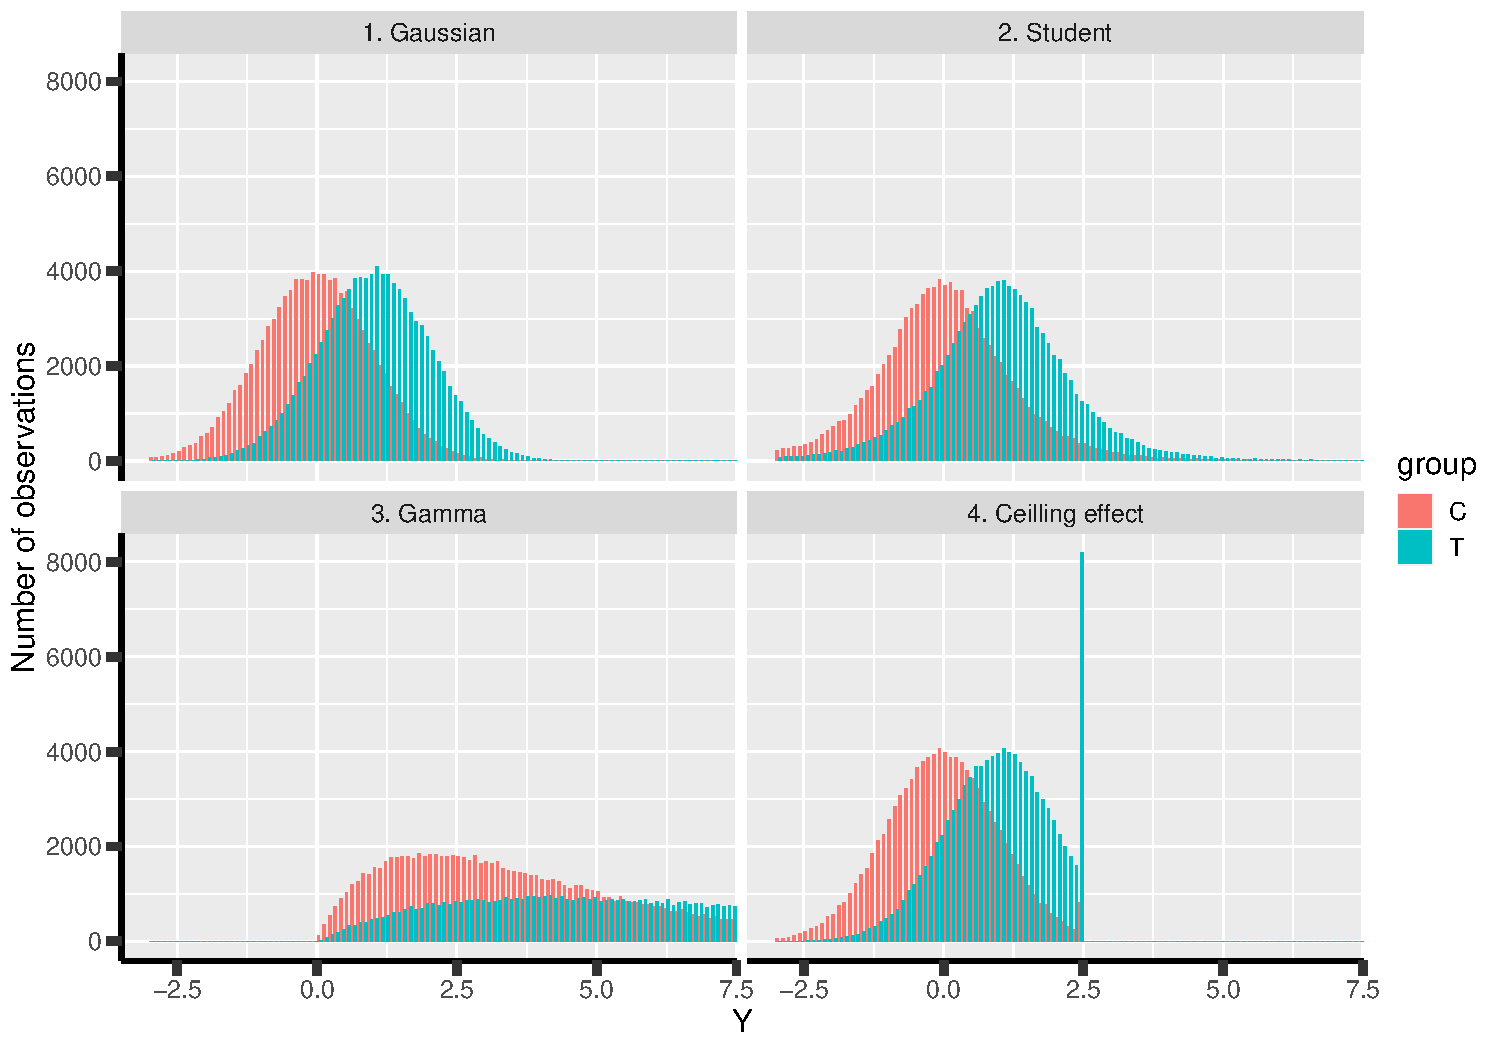
\includegraphics[width=\textwidth]{./figures/examples-hist.pdf}
\caption{\label{fig:examples}Example datasets.}
\end{figure}

\Warning if any, distributional assumptions are usually made on the resiudal terms, e.g:
\begin{align*}
Y = X \beta + \varepsilon \text{ where } \varepsilon \sim \Gaus[0,\sigma^2]
\end{align*}


and not on the outcome \(Y\). Concretely, we don't assume that the
outcome is normally distributed but that within groups (or once we
remove the group effect) it is normally distributed. In example 1, the
outcome is clearly not normally distributed (it is bimodal) but within
groups it is normally distributed.

\vfill

\clearpage

\section{Statistical properites}
\label{sec:org84b8645}

When we use a statistical procedure to estimate a parameter of
interest (say \(\theta\)), we generally want to report an estimate of
this parameter based on the data we have (denoted
\(\widehat{\theta}\)). We generally also want to report the
uncertainty around this estimate via a confidence intervals (denoted
\(IC_{\widehat{\theta}} = [L_{\widehat{\theta}} ;
U_{\widehat{\theta}}]\)) or report a p-value that reflects whether a
value (say \(\theta_0\)) is compatible with the data at hand. We will
therefore distinguish three properties for a statistical procedure:
\begin{itemize}
\item \textbf{validity of the estimate}: the estimate should tend to the true
value as we increase the sample size (consistency) or the average
estimate should tend to the true value as repeat the
experiment (unbiasedness).
\item \textbf{validity of the uncertainty}: the confidence interval should have
proper coverage, typically they should contain the true value with
probablity 95\%. The p-value should have a uniform distribution under
the null meaning that the type 1 error is controlled at its nominal
level, typically 5\%.
\item \textbf{efficiency}: the procedure is optimal in the sense that it makes
the best use of the data at hand. \newline For instance we expect
the estimates to be as precise as possible, i.e. to have the
narrowest possible confidence intervals. We also expect that the
type 2 error should be the smallest possible (i.e. highest
power). In other terms, whenever the null hypothesis is false, the
test should rejected it as often as possible.
\end{itemize}

\bigskip

In the following we will assume that these properties are of
decreasing interest: having unbiased estimates is the most important
as quantifying uncertainty and efficiency can be fixed by
replicating studies and performing a meta-analysis. A non-efficient
estimator can still give useful and valid results - it will "just"
waste ressources but not be misleading (if used and interpreted
correctly).

\clearpage

\section{Should we worry about normality?}
\label{sec:orge958418}

Most statistical procedures do not require any normality assumption to
provide consistent estimates with asymptotically valid confidence
intervals and p-values. For instance t-tests and linear regressions
can be shown to provide consistent and asymptotically normally
distributed estimates in large iid \footnote{independent and identically
distributed} samples, regardless to whether they are normally
distributed as soon as their first two moments are finite. Here it is
important to distringuish between the distribution of the outcome (say
\(Y\)) and the distribution of the parameter of interest, often the
mean of \(Y\). Averaging "normalizes" the distribution, which is
formalized in the central limit theorem, and illustrated on
\autoref{fig:distAverage}:

\begin{figure}[!h]
\centering
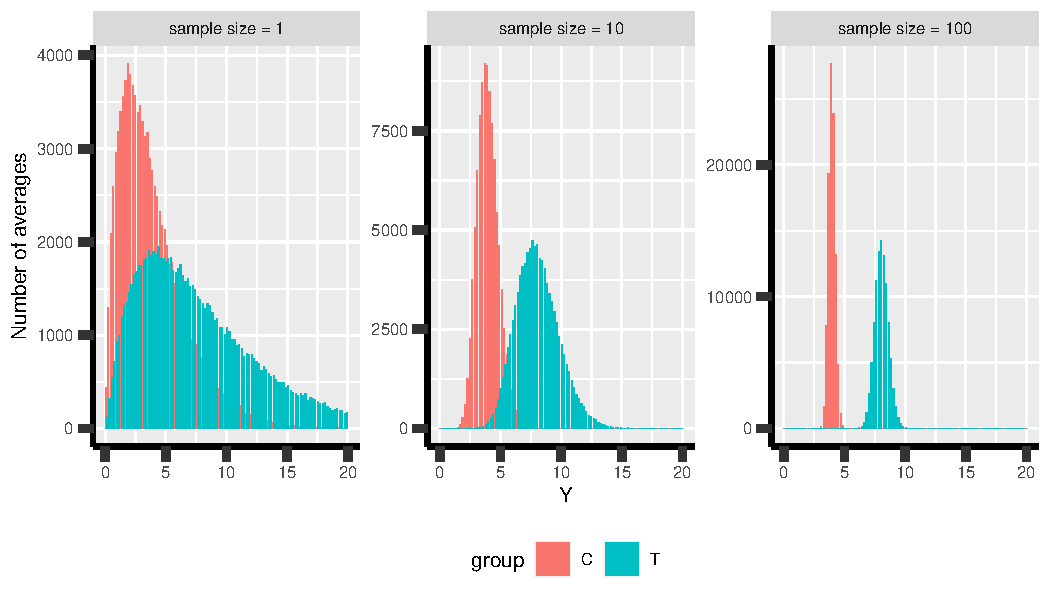
\includegraphics[width=\textwidth]{./figures/examples-histAverage.pdf}
\caption{\label{fig:distAverage}Distribution of the estimated mean along the sample size.}
\end{figure}

This means that (almost) regardless to the input data, we will be able
to estimate parameters which follows a normal distribution, i.e. for
which we can quantify the uncertainty. Results from the M-estimation
theory or the maximum likelihood theory can be used to show that
finding parameters that minimize an error that is the lack of fit
relative to individual observations lead to consistent
estimates. Concretely, this means that the coverage/type 1 error
control of many standard procedures such as the t-test and the linear
regression will be at their nominal level in large samples, even
though the normality assumption is not fullfilled
(\autoref{fig:coverage}) \ldots for large enough sample sizes.

\clearpage

Does that mean we should not worry about normality? No:
\begin{enumerate}
\item we may have a valid test / consistent estimate of a meaningless
parameter.
\item we may only have a small sample.
\item our estimator may not be efficient. This is usually not a problem,
except when we loose so much efficiency that the estimate becomes
very variable. This typically happen in presence of outliers.
\item no assuming normality complicates the understanding the group
effect, as the normal distribution is one of the few distribution
that can be summarized by two, easily interpretable, independent,
parameters (mean and variance).
\item no assuming normality complicates other diagnostic tests, e.g.
correlation is not independence and mean
\end{enumerate}
In the following we will focus on issue 1-3.

\begin{figure}[!h]
\centering
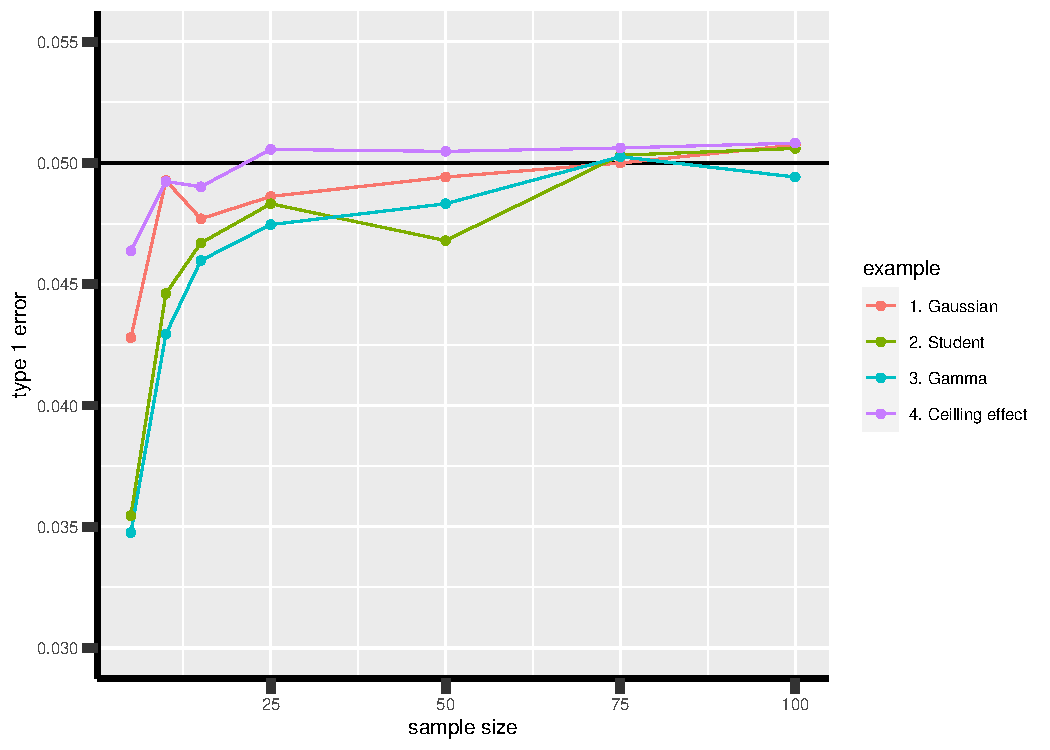
\includegraphics[width=\textwidth]{./figures/examples-coverage.pdf}
\caption{\label{fig:coverage}Coverage of the t-test.}
\end{figure}



\clearpage

\section{Issue 1: parameter of interest with non-normal data}
\label{sec:org6ae3e82}

By default, we generally use the mean to define our parameter of
interest. In our example the difference in mean between the two groups
meaning that we summarize the distribution of the outcome for each
group by its mean (or expected value) and then take the difference
between groups. This is somehow arbitrary, we could have used another
summary statistic like the standard deviation, the median (or any
other quantile), the mode, \ldots. However it is not completely arbitrary:
\begin{itemize}
\item it is \textbf{convenient} to model and compute: many estimators and softwares
have been developped for modeling the mean. Also this can be done
in a numerically stable and efficient way.
\item it is a \textbf{natural} choice if the outcome is normally distributed as
the mean and the variance fully characterize the distribution so no
need to model other summary statistics. In particular, for normal
distributions the mean is equal to the median and the mode of the
distribution.
\item it is \textbf{easy to interpret} if the outcome is normally distributed as
it is the average but also most likely value.
\end{itemize}

When the distribution is not normal, the last two arguments might not
be true. While they approximately hold if the distribution is unimodal
and symmetric, they are not valid for asymetric or bimodal
distribution. For instance, the mean of a binary variable will
correspond to a value that is never observed! If we look at
\autoref{fig:mmm}, we can see that the mean is far from being the most
likely value (i.e. the mode). The median is slightly closer to the
mode but does not really provide a satisfactory improvement. 

\clearpage

\begin{figure}[!h]
\centering
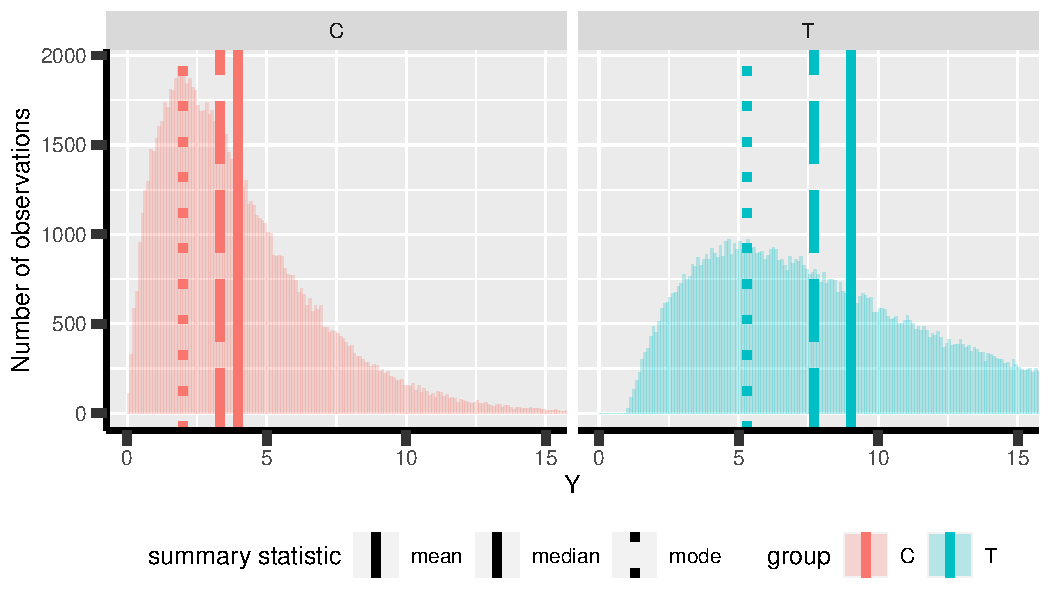
\includegraphics[width=\textwidth]{./figures/meanMedianMode.pdf}
\caption{\label{fig:mmm}Mean, median, and mode two asymetric distributions.}
\end{figure}


 In such a case, it can be a good idea to define a new parameter of
interest. One could for instance apply a transformation that
normalizes the distribution (e.g. log-transformation, see \autoref{fig:logmean}), estimate the
mean of the transformed data (here 1.1 vs 1.8), and compare them
across groups (here 0.7). In the case of a log-transformation, the
back-transformed difference and get a nice interpretation has a nice
interpration: it is a multiplicative effect (exp(0.7)=2, i.e. the mean
in the treatment is twice larger than in the control group). So,
instead of studying an additive group effect (on the mean), the parameter of
interest is a multiplicative group effect (on the mean).


\clearpage

\begin{figure}[!h]
\centering
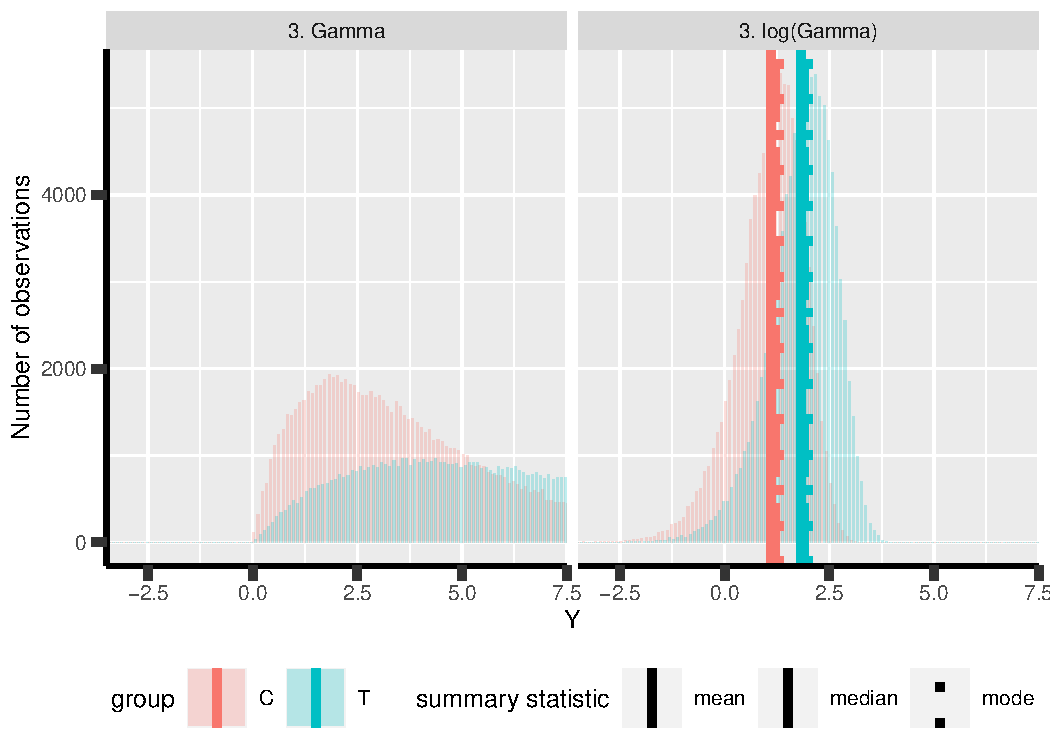
\includegraphics[width=\textwidth]{./figures/logmean.pdf}
\caption{\label{fig:logmean}Mean, median, and mode on the log-transformed data}
\end{figure}


TODO: Mann-Whitney parameter (e.g. if one cannot find a good transformation), Zero inflated model (example 4)

\clearpage

\section{Issue 2: handling small samples with non-normal data}
\label{sec:orgb081a90}

Bias correction

Permutation tests

Robust standard error




\clearpage

\section{Issue 3: handling outliers}
\label{sec:org8cb9ab4}

No good solution here.
Check the influence of each observation. Median more robust than mean.



\section{References}
\label{sec:org0cd96a4}
\begingroup
\renewcommand{\section}[2]{}
\bibliographystyle{apalike}
\bibliography{bibliography}

\endgroup
\end{document}